\section{Survivability of small populations}
\label{sec:small-populations}

The previous sections fixed the mean growth regime and the quasi-stationary picture on survival. Here the question is different, and more directly applied: how does the \emph{initial} count change the chance that a branching population is still alive at a large generation? The answer, in short, is that near criticality survival probabilities are highly sensitive to the initial cohort size $k$---and that sensitivity is a principal reason why stochastic branching, and later birth--death--catastrophe models, matter for early infection at all.

\subsection{Initial cohort of size $k$}
\label{sec:cohort-k}

Return to the discrete death-or-division process with division probability $p$, and write ${}_1u_n$ for the extinction probability by generation $n$ starting from a single individual, so that ${}_1S_n=1-{}_1u_n$. If the process instead starts from $k$ independent founders, extinction by generation $n$ requires every lineage to have died out:
\[
\pr{\text{extinction by }n\mid \zz_0=k}
=
\bigl({}_1u_n\bigr)^k.
\]
Hence the survival probability is
\begin{equation}
\label{eq:Sk}
S_n^{(k)}
=
1 - \bigl({}_1u_n\bigr)^k,
\end{equation}
which for $k>1$ is strictly larger than ${}_1S_n$. The size of the gain is easiest to read as a ratio,
\[
\frac{S_n^{(k)}}{{}_1S_n}
=
\sum_{j=0}^{k-1}\bigl({}_1u_n\bigr)^j
\leq k,
\]
and this ratio approaches its ceiling $k$ whenever ${}_1u_n\to 1$---that is, at late times in the subcritical regime, or wherever survival decays slowly near criticality. Founders then contribute almost independently, and the gain is close to proportional in $k$.

\begin{figure}[ht]
\centering
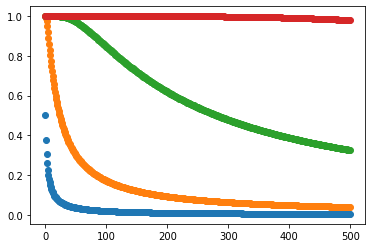
\includegraphics[width=0.65\textwidth]{figures/IMG_ch3/kvals.png}
\caption{Survival probability out to $500$ generations for initial counts $k\in\{1,10,100,1000\}$ (blue through red), at criticality $p=\tfrac12$.}
\label{fig:kvals}
\end{figure}

\begin{figure}[ht]
\centering
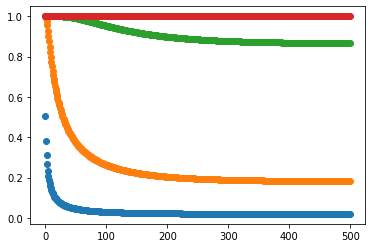
\includegraphics[width=0.45\textwidth]{figures/IMG_ch3/kvals505.png}
\hfill
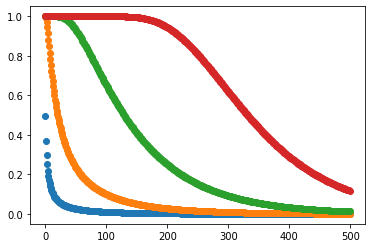
\includegraphics[width=0.45\textwidth]{figures/IMG_ch3/kvals495.png}
\caption{As in Figure~\ref{fig:kvals}, but slightly supercritical ($p=0.505$, left) and slightly subcritical ($p=0.495$, right). The gain from larger $k$ is strongest near $p=\tfrac12$.}
\label{fig:kvals-near}
\end{figure}

Figures~\ref{fig:kvals} and~\ref{fig:kvals-near} show $S_n^{(k)}$ through $500$ generations. Raising $k$ lifts the whole survival curve, and the effect is itself highly sensitive to criticality: it strengthens as $p$ approaches $\tfrac12$ and remains strong just into the supercritical regime. Continuous time carries the same qualitative message, and for the same reason. For independent linear birth--death lineages the extinction probability with $N$ founders is $\bigl(p_0^{(1)}(t)\bigr)^N$, so survival is $1-\bigl(p_0^{(1)}(t)\bigr)^N$, again monotone in the founding count and again sharply dependent on it near criticality.

\subsection{Reading for early infection}
\label{sec:k-infection}

Suppose an infection is only slightly supercritical, or spends an early window near criticality. A modest increase in the founding inoculum can then change the odds of persistence far more than a naive proportional reading of the mean would suggest. Mechanisms that raise the effective early count---a sheltered intracellular burst before extracellular exposure, for example---are therefore natural candidates for selective advantage even when the later per capita rates are entirely unchanged. The present section records only the branching-process mechanism behind that reading; the pathogen life histories in which it is realised are taken up in later chapters.

\subsection{Teaser: discrete birth--death--catastrophe}
\label{sec:bdc-teaser}

A discrete-time birth--death--catastrophe (BDC) process adds, at each generation, a chance that the whole population is removed by a catastrophe event such as a rupture, on top of the ordinary death and division already in place.

Suppose each individual independently triggers catastrophe with probability $\kappa$ when the count is $n$, so that the probability of no catastrophe in that generation is $(1-\kappa)^n$. Because this survival factor depends on the current size, surviving paths are reweighted by a quantity that depends on the whole trajectory of sizes rather than on its endpoint. The law conditional on avoiding catastrophe is consequently \emph{not} the plain Galton--Watson law of Section~\ref{sec:qs-discrete}, and the conditional mean is not simply $1/A(p)$.

None of that takes the model out of reach. One can still read the construction as a size-dependent thinning of the offspring mechanism: the process remains in the branching family, and quasi-stationary ideas continue to apply, though with constants that now depend on $\kappa$. In a pure birth--catastrophe caricature with no death, counts are deterministic between ruptures and several probabilities are elementary; restoring death makes them random again. The full continuous-time, rate-based bookkeeping is the subject of the birth--death--catastrophe chapters. For Path~A it is enough that small-$k$ survival and carefully conditioned quasi-stationarity remain the organising motifs once catastrophes are present.
